\documentclass[a4paper,11pt]{article}

\usepackage[T1]{fontenc}

\usepackage[utf8]{inputenc}

\usepackage[italian]{babel}

\usepackage{graphicx}

\usepackage{indentfirst}

\usepackage{amsmath,amssymb}

\usepackage{enumitem} 

\newcommand{\virgolette}[1]{``#1''}

\usepackage[margin=1in]{geometry} %Smaller margins

\usepackage{lmodern} %Vector PDF

\usepackage{siunitx}

\usepackage{xcolor}

\usepackage{colortbl}

\usepackage{multirow}

\usepackage{rotating}

\usepackage{booktabs}

\usepackage{longtable}

\usepackage{graphicx}
\graphicspath{ {../../Immagini/} }

\usepackage{wrapfig}

\usepackage{siunitx} % Per unit� di misura in generale e la corretta rappresentazione dei numeri.

\usepackage{gensymb} % Per il simbolo di gradi

\begin{document}

	\begin{abstract}

	Questo documento contiene la procedura e l'analisi dati di un esperimento volto a misurare la velocità della luce. Tra i tanti metodi architettati per calcolare tale costante, in questo esperimento si è seguito il metodo di Foucault, che rende l'analisi dati relativamente semplice. L'approccio di questo documento al problema suddetto è rigorosamente scientifico e statistico.

	\end{abstract}

	\section{Introduzione}
	
	\begin{wrapfigure}{r}{0.5\textwidth}
    	\centering
    	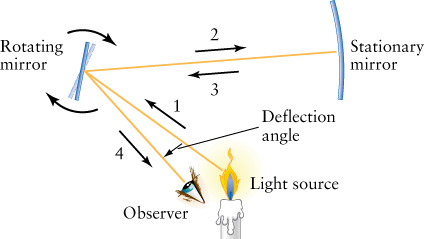
\includegraphics[width=0.5\textwidth]{Apparato}
    	
    	\label{apparato}
    	\caption{Schema semplificato dell'apparato}
	\end{wrapfigure}	
	
	Il fine di questo esperimento è quello di misurare una delle costanti dell'universo, la velocità della luce $c$. Il problema è stato storicamente affrontato in maniere diverse e, passando per una ridefinizione delle unità di misura, si è giunti al valore noto ed esatto di $c = \SI{299792458}{\meter / \second}$. Questo valore subisce una correzione per via del mezzo in cui avviene l'esperimento: l'aria.
	Il metodo qui seguito è quello di Focault, che permette di eseguire l'esperimento in spazi ridotti e richiede un'analisi dati relativamente semplice. Il principio di funzionamento è riassunto in maniera semplificata nell'immagine \ref{apparato}. Il principale strumento dell'esperimento è un piccolo specchio rotante, con alta velocità di rotazione (intorno ai $\SI{1000}{rad / s}$). La sorgente di luce, un laser con lunghezza d'onda di approssimativamente $\SI{633}{\nano \meter}$, incide sullo specchio rotante. Quando questo si trova ad un angolo preciso, la luce riflessa va ad incidere su uno specchio concavo e torna indietro. Nel tempo che la luce è andata e tornata sullo specchio rotante esso ha compiuto una rotazione di un angolo facilmente calcolabile (per i dettagli si veda la sezione sulla procedura), che ovviamente varierebbe se la luce avesse una velocità diversa. Osservando il punto di ritorno si può calcolare tale angolo e da esso si trova la velocità della luce.
	Quella appena esposta è una versione assai semplificata per capire il funzionamento dell'esperimento. In realtà, per ridurre le dimensioni dell'apparato sperimentale, il percorso che la luce compie avanti e indietro una volta riflessa dallo specchio rotante viene allungato tramite una riflessione su tre specchi concavi, come si può vedere nelle immagini delle sezioni successive e il raggio viene focalizzato attraverso due lenti opportunamente posizionate. La misura viene fatta grazie a uno specchio semiargentato che lascia passare la luce che poi andrà a incidere sullo specchio rotante ma che riflette quella che torna, che viene poi vista attraverso un oculare. Poiché è piuttosto ovvio che la luce viene deviata tanto più alta è la velocità di rotazione, la misura può essere fatta confrontando la posizione del raggio riflesso con basse velocità di rotazione (circa $\SI{100}{rad / \second}$) con quella del raggio ad alte velocità di rotazione (oltre $\SI{1000}{rad / \second}$).
	

\end{document}